% This is "sig-alternate.tex" V2.0 May 2012
% This file should be compiled with V2.5 of "sig-alternate.cls" May 2012
%
% This example file demonstrates the use of the 'sig-alternate.cls'
% V2.5 LaTeX2e document class file. It is for those submitting
% articles to ACM Conference Proceedings WHO DO NOT WISH TO
% STRICTLY ADHERE TO THE SIGS (PUBS-BOARD-ENDORSED) STYLE.
% The 'sig-alternate.cls' file will produce a similar-looking,
% albeit, 'tighter' paper resulting in, invariably, fewer pages.
%
% -----------------------------------------------------------------------------
% This .tex file (and associated .cls V2.5) produces:
%       1) The Permission Statement
%       2) The Conference (location) Info information
%       3) The Copyright Line with ACM data
%       4) NO page numbers
%
% as against the acm_proc_article-sp.cls file which
% DOES NOT produce 1) thru' 3) above.
%
% Using 'sig-alternate.cls' you have control, however, from within
% the source .tex file, over both the CopyrightYear
% (defaulted to 200X) and the ACM Copyright Data
% (defaulted to X-XXXXX-XX-X/XX/XX).
% e.g.
% \CopyrightYear{2007} will cause 2007 to appear in the copyright line.
% \crdata{0-12345-67-8/90/12} will cause 0-12345-67-8/90/12 to appear in 
% the copyright line.
%
% -----------------------------------------------------------------------------
% This .tex source is an example which *does* use
% the .bib file (from which the .bbl file % is produced).
% REMEMBER HOWEVER: After having produced the .bbl file,
% and prior to final submission, you *NEED* to 'insert'
% your .bbl file into your source .tex file so as to provide
% ONE 'self-contained' source file.
%
% ================= IF YOU HAVE QUESTIONS =======================
% Questions regarding the SIGS styles, SIGS policies and
% procedures, Conferences etc. should be sent to
% Adrienne Griscti (griscti@acm.org)
%
% Technical questions _only_ to
% Gerald Murray (murray@hq.acm.org)
% ===============================================================
%
% For tracking purposes - this is V2.0 - May 2012

\documentclass{sig-alternate}

\begin{document}
%
% --- Author Metadata here ---
 \conferenceinfo{GECCO'13,} {July 6-10, 2013, Amsterdam, The Netherlands.}
    \CopyrightYear{2013}
    \crdata{TBA}
    \clubpenalty=10000
    \widowpenalty = 10000
%\CopyrightYear{2007} 
% Allows default copyright year (20XX) to be over-ridden - IF NEED BE.
%\crdata{0-12345-67-8/90/01}  
% Allows default copyright data (0-89791-88-6/97/05) to be over-ridden -
% --- End of Author Metadata ---

\title{Compare NSGA-II, SPEA2, MOEA/D Performance for Task Assignment Problem}
%
% You need the command \numberofauthors to handle the 'placement
% and alignment' of the authors beneath the title.
%
% For aesthetic reasons, we recommend 'three authors at a time'
% i.e. three 'name/affiliation blocks' be placed beneath the title.
%
% NOTE: You are NOT restricted in how many 'rows' of
% "name/affiliations" may appear. We just ask that you restrict
% the number of 'columns' to three.
%
% Because of the available 'opening page real-estate'
% we ask you to refrain from putting more than six authors
% (two rows with three columns) beneath the article title.
% More than six makes the first-page appear very cluttered indeed.
%
% Use the \alignauthor commands to handle the names
% and affiliations for an 'aesthetic maximum' of six authors.
% Add names, affiliations, addresses for
% the seventh etc. author(s) as the argument for the
% \additionalauthors command.
% These 'additional authors' will be output/set for you
% without further effort on your part as the last section in
% the body of your article BEFORE References or any Appendices.

\numberofauthors{3} %  in this sample file, there are a *total*
% of EIGHT authors. SIX appear on the 'first-page' (for formatting
% reasons) and the remaining two appear in the \additionalauthors section.
%
% There's nothing stopping you putting the seventh, eighth, etc.
% author on the opening page (as the 'third row') but we ask,
% for aesthetic reasons that you place these 'additional authors'
% in the \additional authors block, viz.
% Just remember to make sure that the TOTAL number of authors
% is the number that will appear on the first page PLUS the
% number that will appear in the \additionalauthors section.

\maketitle
\section{Description}
The aim of these experiments is to explore the multiobejctive algorithms framework (e.g. jMetal, MOEA, or any other) and identify the most effective multi-objective algorithm, which gives an approximation set to the Pareto front of the problem with best convergence and uniform diversity




\section{Problem Formulation}
\label{sec: model}
In this section, we describe our problem formulation which is an extension of 
the problem defined by Younas et al.~\cite{irfan2011}. The problem discussed 
in this paper deals with multi-objective optimal assignment of tasks to 
collaborating teams of agents.
Let $\mathcal{A} = \{a_i|i=1, \dots, m\}$ be the set of $m$ agents 
(candidate members) and let $\mathcal{T} = \{t_j|j=1, \dots, n\}$ be the set 
of $n$ tasks, where $m \geq n$. 
Each agent $a_i \in \mathcal{A}$ has a set of $p$ 
attributes $c_i = \{c_{ik}|k=1, \dots, p\}$, which are real values that 
quantify its capabilities. Similarly for each task $t_j \in \mathcal{T}$, 
a weight is associated to each capability and it defines 
capability weight vector $w_j = \{w_{kj}|k=1, \dots, p\}$. Assume that each 
task $t_j$ requires a team of agents with a fixed 
number $b_{j}$ of agents. 
Each agent $a_i \in \mathcal{A}$ can perform at most one task.
We denote the team of $b_j$ agents performing task $t_j$ by
$team_{_{\mathcal{S}_j}}$, where the index $\mathcal{S}_j$ is a set
\begin{equation*} 
\mathcal{S}_j \subset \{1, 2, \dots m\}, 
\quad |\mathcal{S}_j| = b_j, \quad a_i \in team_{_{\mathcal{S}_j}} 
\Leftrightarrow i \in \mathcal{S}_j.
\end{equation*}

We also assume that total completion time for each task $t_j$ 
is $time_j$ (time units), in our case $time_j$ represent number of hours 
required to perform task $t_j$. 
Assuming each agent $a_i \in \mathcal{S}_j$ participating in $team_j$ works 
for equal $\left(\frac{time_j}{b_j}\right)$ number of hours on task $t_{j}$. 
Each agent $a_i$ has a salary $Salary_i$, which is a function of its 
capabilities and certain weights (values) for those 
capabilities $h(c_{ik}, v_{k}|k=1, \dots, p)$, where $v_{k}$ defines relative 
value for capability $k$ for calculating salary. 
Within each team, agents collaborate with each other which improve the 
quality of the task performed. 
The execution of each task also incurs some cost which depends on completion 
time and salary of the agents assigned to the task.


The goal is to optimally assign all tasks to teams of agents such that quality 
is maximized and cost is minimized. Now we proceed to models for calculating 
these two objectives, the quality and the cost.

\subsection{Model for quality calculation}
We assume that agents participating in a team collaborate within team 
environment and they produce value (quality) which is a non-linear function of 
these agents and the assigned task. 
Thus $team_{_{\mathcal{S}_j}}$, which performs 
task $t_j$ produces the quality $f(team_{_{\mathcal{S}_j}}, t_j)$. 
In order to calculate the quality, we consider the team-working model 
introduced in~\cite{irfan2011} which is an extension of the base model 
introduced in~\cite{kamrani2009} and~\cite{kamrani2010}. 
The overall quality of performing all tasks is defined as sum of values 
produced by the teams. One of the objectives is to maximize the 
quality i.e., maximizing the objective function
\begin{equation}\label{equ: objective}
\mathcal{Z}_1(\mathcal{S}_1, \dots \mathcal{S}_n) 
= \sum_{j=1}^n f({team_{_{\mathcal{S}_j}}, t_j}).
\end{equation}

An agent in a team may be influenced by the capabilities of other 
participating agents. The quality produced by a team is assumed to be equal 
to the sum of values produced by the participating agents:
\begin{equation}\label{equ: value_function}
  f(team_{_{\mathcal{S}_j}}, t_j) = \sum_{i \in \mathcal{S}_j} 
  q(a_i, team_{_{\mathcal{S}_j}}, t_j).
\end{equation}

If a task is performed by a single agent, then quality produced by the agent 
is equal to weighted sum of the agents capabilities, i.e.,
\begin{equation}\label{equ: single}
  q(a_i, t_j) = \sum_{k=1}^p c_{ik} w_{kj}. 
\end{equation}  

However, if a task is performed by a team, the agents are influenced by other 
team members and capability of each type is influenced by maximum 
capability $(c_k^{\max})$ of that type. 
The new capabilities are calculated as
\begin{equation}\label{equ: boost} 
  c_{ik}' = c_{ik} + \frac{c_{ik}(c_k^{\max}-c_{ik})}{c_k^{\max}},
\end{equation}
where $c_k^{\max}  =\underset{i \in \mathcal{S}_j}{\max} \{c_{ik}\}, 
\quad \forall k \in \{1, \dots, p\}.$ 

Equation (\ref{equ: boost}) indicates the following:
\begin{enumerate}
\item A capability $c_{ik}$ of an agent ${a_i}$ improves only when its value is 
  less than the maximum capability $c_k^{\max}$ of that type in a team. 
  Thus the agents with such capabilities benefit from the team working. 
\item A capability $c_{ik}$ of an agent ${a_i}$ where $c_{ik} = c_k^{\max}$ is not 
  affected by collaboration.
\item A capability $c_{ik} = 0$ of an agent ${a_i}$ is not affected by team 
  collaboration.
\item A capability $c_{ik}$ of an agent ${a_i}$ 
  where $c_{ik}=\frac{c_k^{\max}}{2}$ has the highest improvement due to 
  collaboration. 
\end{enumerate}

From equation (\ref{equ: single}) and (\ref{equ: boost}), the quality achieved 
by an agent while working and collaborating with other team members is 
obtained as
\begin{equation}\label{equ: team}
  q(a_i, team_{_{\mathcal{S}_j}}, t_j) = 
  \sum_{k=1}^p (c_{ik} 
  + \frac{c_{ik}(c_k^{\max}-c_{ik})}{c_k^{\max}})w_{kj}. 
\end{equation}

By substituting (\ref{equ: team}) and (\ref{equ: value_function}) 
into the objective function (\ref{equ: objective}), we get the 
following final quality function:  
\begin{equation}\label{equ: objective4}
  \mathcal{Z}_1 = \sum_{j=1}^n\sum_{i=1}^m \sum_{k=1}^p (c_{ik} 
  + \frac{c_{ik}(c_k^{\max}-c_{ik})}{c_k^{\max}})w_{kj}x_{ij}, 
\end{equation}
where $c_k^{\max} = 
\underset{ 1 \leq i \leq m }{\max} \{c_{ik} x_{ij}\}$\\ 
and \mbox{$x_{ij} = 1$} if task $t_j$ is assigned to agent $a_i$ and $0$ 
otherwise.

\subsection{Model for cost calculation}
The cost of performing a given task $t_j$ depends on the capabilities 
$(c_l = \{c_{l1}, \dots, c_{lp}\}, \quad \forall l \in \mathcal{S}_j)$ of 
assigned agents and the estimated completion time $time_j$. 
Each agent $a_i$ has a salary $Salary_i$, which is a function of its 
capabilities and certain weights (values) for those 
capabilities $h(c_{ik}, v_{k}|k=1, \dots, p)$, where $v_{k}$ defines relative 
value for capability $k$ for calculating salary. 

The overall cost is defined as the sum of the costs of performing all given 
tasks. 
Our objectives is to minimize the cost i.e., minimizing the objective function
\begin{equation}\label{equ: cost-objective}
\mathcal{Z}_2(\mathcal{S}_1, \dots \mathcal{S}_n) 
= \sum_{j=1}^n g({team_{_{\mathcal{S}_j}}, t_j}).
\end{equation}

Here $g$ is the cost function
\begin{equation}\label{equ: cost_function}
  g(team_{_{\mathcal{S}_j}}, t_j) = \sum_{i \in \mathcal{S}_j} 
  cost(a_i, team_{_{\mathcal{S}_j}}, t_j).
\end{equation}

Moreover, we assume that all assigned agents to a task work for the same 
duration (equal number of hours). The cost of a single agent $a_i$ assigned to 
a task $t_j$ is calculated as:
\begin{equation}\label{equ: cost_agent}
  cost(a_i, team_{_{\mathcal{S}_j}}, t_j) = Salary_i(\frac{time_j}{|\mathcal{S}_j|}).
\end{equation}

Salary of an agent $a_i$ is defined by
\begin{equation}\label{equ: salary_agent}
  Salary_i = h(c_{ik}, v_{k}), \forall k \in \{1, \dots, p\},
\end{equation}
where $v_{k}$ defines relative value for capability $k$. We use a simple model 
here and estimate the salary as the weighted sum of the capabilities, i.e. 
$h(c_{ik}, v_{k}) = \sum_{k=1}^p c_{ik} v_{k}.$ 

By substituting (\ref{equ: salary_agent}) 
and (\ref{equ: cost_function}) into the objective function 
(\ref{equ: cost-objective}), we get the following final cost function:

\begin{equation}\label{equ: final_cost_objective}
  \mathcal{Z}_2 = \sum_{j=1}^n (\frac{time_j}{|\mathcal{S}_j|} 
  \sum_{i=1}^m \sum_{k=1}^p c_{ik}v_{k}x_{ij}), 
\end{equation}
where \mbox{$x_{ij} = 1$} if task $t_j$ is assigned to agent $a_i$ 
and $0$ otherwise.


\subsection{A Multi-Objective Model with Constraints}
In this section, we present a bi-objective model with constraints. 
Our goal is to maximize quality and minimize cost while assigning all given 
tasks to collaborating teams of agents. Mathematical formulation is summarized 
as follows:

\begin{equation}\label{equ: quality-objective-overall}
  Maximize \quad \mathcal{Z}_1 = \sum_{j=1}^n\sum_{i=1}^m \sum_{k=1}^p (c_{ik} 
  + \frac{c_{ik}(c_k^{\max}-c_{ik})}{c_k^{\max}})w_{kj}x_{ij}, 
\end{equation}

\begin{equation}\label{equ: cost_objective_overall}
  Minimize \quad \mathcal{Z}_2 = \sum_{j=1}^n (\frac{time_j}{|\mathcal{S}_j|} 
  \sum_{i=1}^m \sum_{k=1}^p c_{ik}v_{k}x_{ij}), 
\end{equation}

subject to constraints
\begin{equation}\label{cons: one_task}
  \sum_{j=1}^n x_{ij} = 1, \hspace{18pt}  
  \forall a_i \in \mathcal{A} \hspace{41pt} 
\end{equation}

\begin{equation}\label{cons: group_size}
\sum_{i=1}^m x_{ij} = b_j,\hspace{13pt}
 \forall t_j \in \mathcal{T}\hspace{42pt} 
\end{equation}

\begin{equation}\label{cons: least_one_agent}
  b_j \geq 1, \hspace{37pt}  \forall t_j \in \mathcal{T} \hspace{41pt}
\end{equation}

\begin{equation}\label{cons: agents_nr}
  \sum_{j=1}^n b_j \leq m \hspace{96pt}
\end{equation}

\begin{equation}\label{cons: one_zero}
  x_{ij} \in \{0,1\}, \hspace{15pt} \forall a_i \in \mathcal{A},\, 
  \forall t_j \in \mathcal{T}
\end{equation}
where \mbox{$b_j=|\mathcal{S}_j|$}, $\mathcal{S}_j$ is a set of assigned 
agents to task $t_j$. Constraint (\ref{cons: one_task}) states that an agent 
can perform at most one task. Constraint (\ref{cons: group_size}) ensures that 
each task $t_j$ is performed by a $team_{_{\mathcal{S}_j}}$, which consists 
of $b_j$ agents. 
Constraint (\ref{cons: least_one_agent}) means that 
each $team_{_{\mathcal{S}_j}}$ should have at least one agent and 
constraint (\ref{cons: agents_nr}) ensures that number of agents assigned to 
all $n$ teams should be equal or less than total number of available 
agents $m$. The last constraint (\ref{cons: one_zero}) is an assignment matrix,
where $x_{ij}=1$ means task $t_j$ is assigned to agent $a_i$.




\section{Problem Instances (Data Set)}\label{sec: experiments}


\begin{table*}[ht!]
\scriptsize
\caption{Specification of the Collaborating Teams Assignment Problem Instances}
\centering

\begin{tabular}{p{0.30in} p{0.49in} p{0.49in} p{0.50in} p{4.2in}}
  \hline\hline
  Prob\# & Total Agents & Required Agents&  Number of Tasks &  
  Teams (\# of agents assigned to the tasks)  \\ [0.5ex] % inserts table
  \hline 
  1 & 10 & 10 & 4 & [2, 3, 2, 3]  \\ 
  2 & 50 & 20 & 4 & [3, 4, 6, 7]  \\
  3 & 400 & 400 & 100 & 100 teams (each team has 4 agents)  \\
  \hline
\end{tabular}
\label{table:teamsFormulationDataSet}
\end{table*}


In order to make the analysis and discussion unbiased, we consider 
more than one instances of collaborating teams assignments with different 
problem sizes as shown in Table~\ref{table:teamsFormulationDataSet}. In all 
problem instances, each agent $a_i$ has $10$ different 
capabilities $c_i = \{c_{ik}|k=1, \dots, 10\}$ and each task $t_j$ has certain 
requirements (weights) $w_j = \{w_{kj}|k=1, \dots, 10\}$ for 
these capabilities. We assume that the values of $c_{ik}$ and $w_{kj}$ are 
integer values between $0$ and $4$ inclusive, where $0$ is the lowest and $4$ 
is the highest value for the agent's capability and the capability's weight 
for the task. 
Assuming that most of the agents have average capability values and most 
of the tasks require average capabilities, we generate 
input data with smaller probabilities to extreme values and higher 
probabilities to average values. The synthetic data is generated randomly such 
that $p(c_{ik}=4.0) = 0.1, p(c_{ik}=3.0) = 0.15, p(c_{ik}=2.0) = 0.5, p(c_{ik}=1.0) = 0.15$ and $p(c_{ik}=0.0) = 0.1$. 
The same distribution is followed while generating weights $w_{kj}$ for the 
task $t_j$. We also assume that total completion time for each task $t_j$ is 
$time_j$ (time units). In our case $time_j$ represents number of hours required 
to perform task $t_j$, which is generated with uniform distribution 
on $[1000 ,1500]$. 
It is assumed that each agent $a_i \in \mathcal{S}_j$, participating 
in $team_j$ works 
for equal $\left(\frac{time_j}{b_j}\right)$ number of hours on task $t_{j}$. 
Each agent $a_i$ has a salary $Salary_i$, which is a function of its 
capabilities and certain weights (values) for those 
capabilities $h(c_{ik}, v_{k}|k=1, \dots, p)$, where $v_{k}$ defines relative 
value for each capability $k$ for calculating salary and we assume $v_{k}=1$ 
for each capability. The execution of each task also incurs some cost, which 
depends on completion time and salary of the resources (agents) assigned to 
the task.

%For all experiments, we have chosen parameters such that they give a fair comparsion between the chosen algorithms (NSGA-II and SPEA2). The initial population size are set %to $20$, $40$, $80$, $160$ and $320$. The algorithms terminate after $100\ 000$ function evaluations. The detail of these parameters is given in %Table~\ref{table:parameterization}.

\subsection{Performance comparison}
To compare and discuss the performance of NSGA-II SPEA2, and MOEA/D a set of computational experiments are performed   with different problem sizes as shown in Table~\ref{table:teamsFormulationDataSet}. NSGA-II SPEA2, and MOEA/D are stochastic in nature and different replications can produce different results. In order to overcome this problem, we consider 10 independent replications for each algorithm and compare the results by considering mean and standard deviation. 
In evolutionary algorithms, initial population size play an important role in the quality of the results. Different algorithms show different behavior on different population sizes. Considering constant number of fitness evaluations, population size can play an important role in evolution. There is some trade-off as far as size of the population is concerned. For example if we assume small population size, then sometimes less number of evaluations may be required for convergence of the population to the Pareto-optimal solutions. But sometimes smaller population can be cause of pre-mature termination (algorithm can be trapped by local minima/maxima). To make the discussion fair, for each problem size, we conduct 10 replications of each algorithm on five different initial population sizes (20, 40, 80, 160 and 320) and each algorithm terminates after 100, 000 function evaluations. For each replication, we calculate the Hypervolume, Spread and GD, and IGD of the obtained Pareto front.

Calculate mean and standard deviation of Hypervolume, Spread and GD, and IGD of 10 replications for each population size.


Example Plot: Draw plots for Hypervolume, Spread and Coverage as shown in Figure 1. You also have to include  curve for MOEA/D.

Example Table: You also need to have tables for  mean and standard deviation of Hypervolume, Spread and GD, and IGD as shown in Table 2.


Reference Pareto front: For each problem, we integrate all obtained nondominated set of solutions for all 10 replications on 20, 40, 80, 160 and 320 initial population sizes. 


Assignment should be done in jMetal5.3 or MOEA Framework or any other available framework, the algorithms are already implemented, you have to explore the framework and perform the experiments.  You need to submit plots with results in tables and the source files.





\begin{table}[h!]
  \caption{Hypervolume Results: (on initial population size = $160$) }
  \centering
  \scriptsize
  %\begin{tabular}{p{0.15in} p{0.24in} p{0.24in} p{0.35in} p{1.8in}}
  \begin{tabular}{p{0.30in} p{0.5in} @{\extracolsep{1cm}}p{0.2in} p{0.4in} 
      p{0.2in}}
    \hline\hline \\
    Prob\# & \multicolumn{2}{p{0.7in}}{NSGA-II} 
    &  \multicolumn{2}{p{0.6in}}{SPEA2} \\[2pt] \cline{2-3} \cline{4-5} \\
    &  $\overline{HV}$ &  $\sigma _{HV}$    & $\overline{HV}$ 
    &  $\sigma _{HV}$   \\ [1pt] % inserts table
    \hline % inserts single horizontal line
    1 & 0.7986 & 0.0 & 0.7986 & 0.0  \\ % inserting body of the table
    2 & 0.8412 & 0.0 & 0.8407 & 0.0032  \\
    3 & 0.5917 & 0.0897 & 0.5176 & 0.0974  \\
    %2 & 2 & 3 & 4 & 50  \\ [1ex] % [1ex] adds vertical space
    \hline %inserts single line
  \end{tabular}
  \label{table:resultsHypervolumePopSize160}
\end{table}




\begin{figure}[h!]
  \centering
  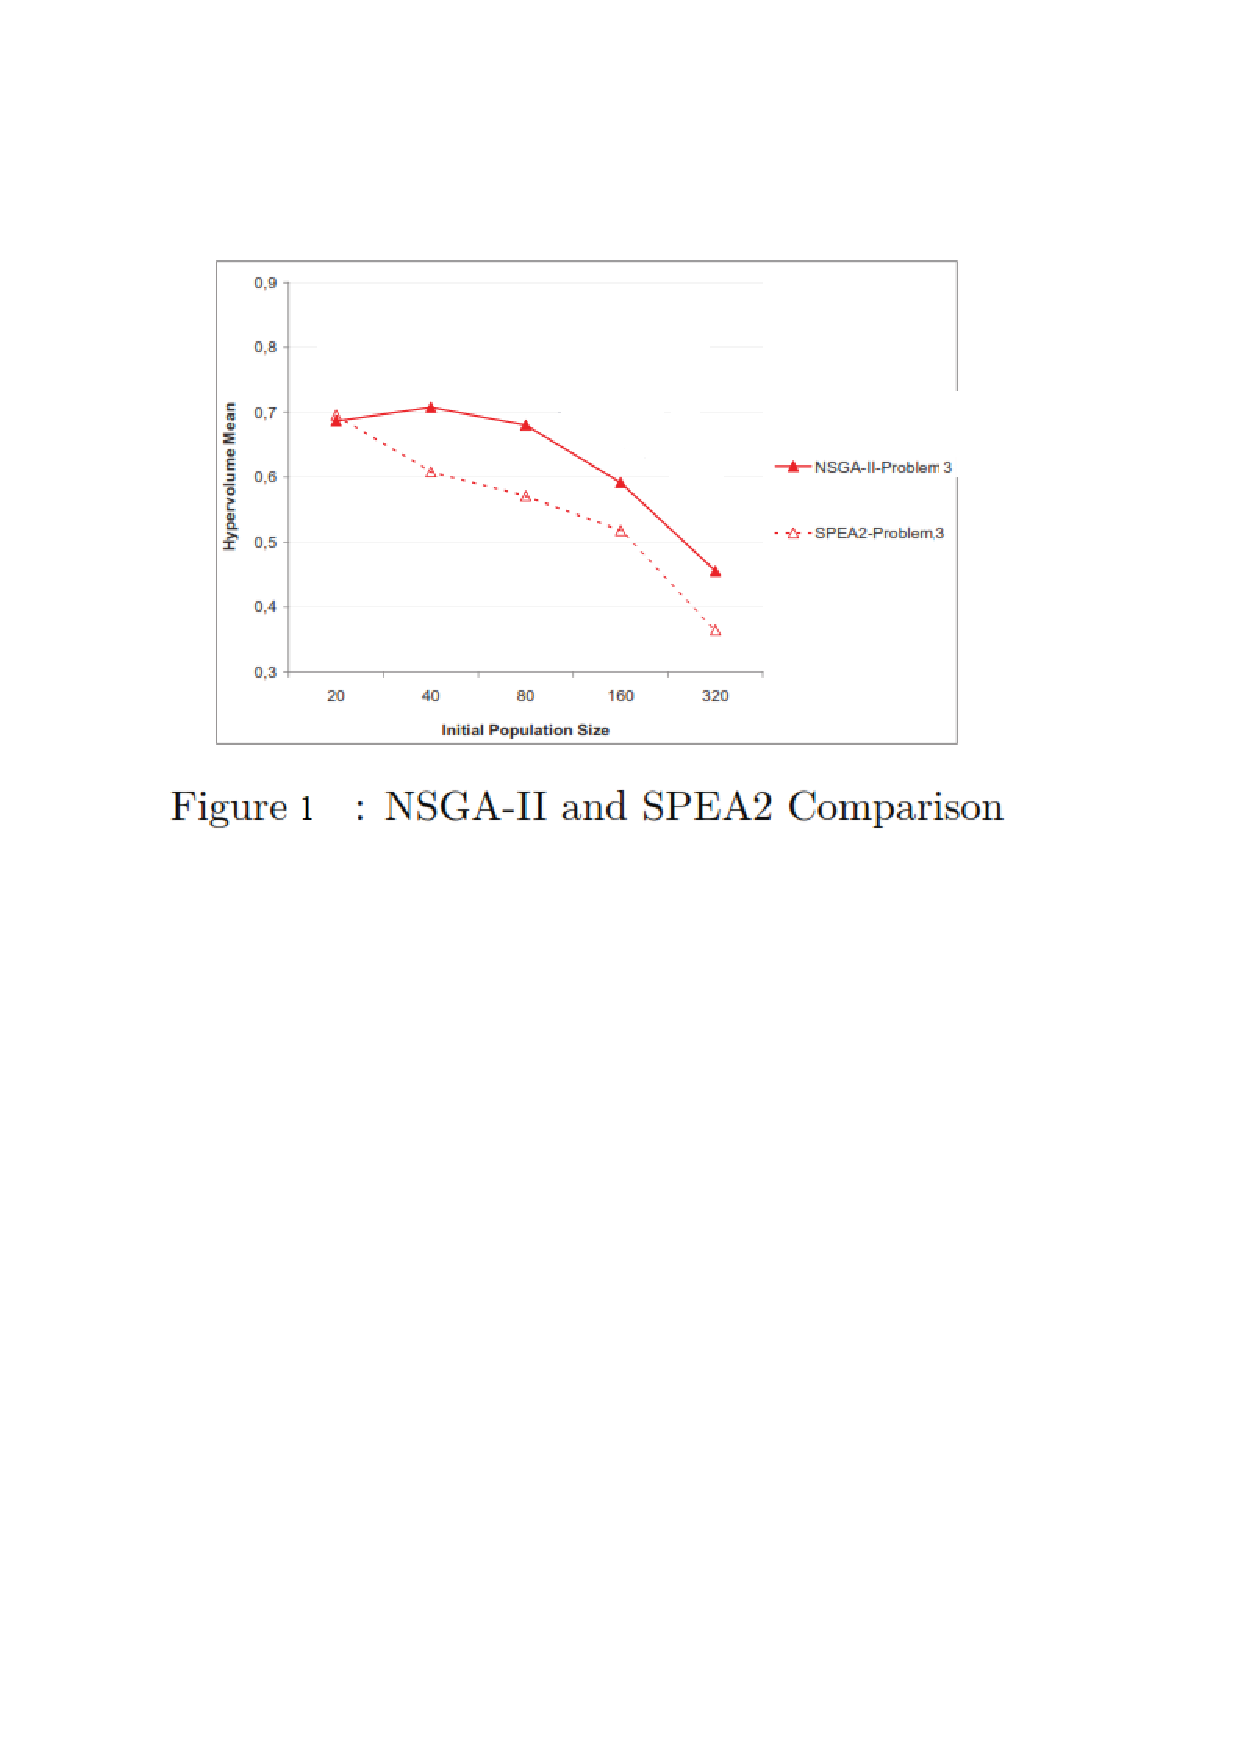
\includegraphics[totalheight=0.23\textheight,width=0.42\textwidth]{algorithmsComparison.png}
  %\includegraphics[scale=0.51,bb=0 0 290 280]{iterationsTime.jpg}
  \caption{NSGA-II and SPEA2 Comparison}
  \label{fig:algorithmsComparison}
\end{figure}


%\end{document}  % This is where a 'short' article might terminate
%
% The following two commands are all you need in the
% initial runs of your .tex file to
% produce the bibliography for the citations in your paper.
%\bibliographystyle{abbrv}
%\bibliography{references}  
% sigproc.bib is the name of the Bibliography in this case
% You must have a proper ".bib" file
%  and remember to run:
% latex bibtex latex latex
% to resolve all references
%
% ACM needs 'a single self-contained file'!
\end{document}
